\subsubsection{05.12.2015 (Competition)}
\textit{\textbf{Time frame:}} 8:00-23:00 

Today there were qualification matches. Our team managed to reach the 2-nd place. \newline
After that there were final matches. There were less than 20 teams in the competition, so the final alliances were consisting of 2 teams each. We chose team PML30-x. Due to nice teamwork our alliance won the competition.

During the matches it was found out, that the robot has a very high center of mass, so it's easy for it to be overturned while climbing the mountain (figure \ref{Overturn1.1}, \ref{Overturn1.2}). So, the robot should be operated more carefully.

\begin{figure}[H]
	\begin{minipage}[h]{0.47\linewidth}
		\center{\includegraphics[scale=0.2]{3Engineering/5Team_meetings/days_of_meetings/2015.12.05/images/01}}
		\caption{Robot is overturned 1}
		\label{Overturn1.1}
	\end{minipage}
	\hfill
	\begin{minipage}[h]{0.47\linewidth}
		\center{\includegraphics[scale=0.2]{3Engineering/5Team_meetings/days_of_meetings/2015.12.05/images/02}}
		\caption{Robot is overturned 2}
		\label{Overturn1.2}
	\end{minipage}
\end{figure}

The elevator didn't work because of no winch, so it was decided to temporarily remove bucket and install the beam, that will be used for scoring alpinists into the shelter and releasing the bottom alpinist at the mountain (figure \ref{Alpinists1.1}, \ref{Alpinists1.2}).

\begin{figure}[H]
	\begin{minipage}[h]{0.47\linewidth}
		\center{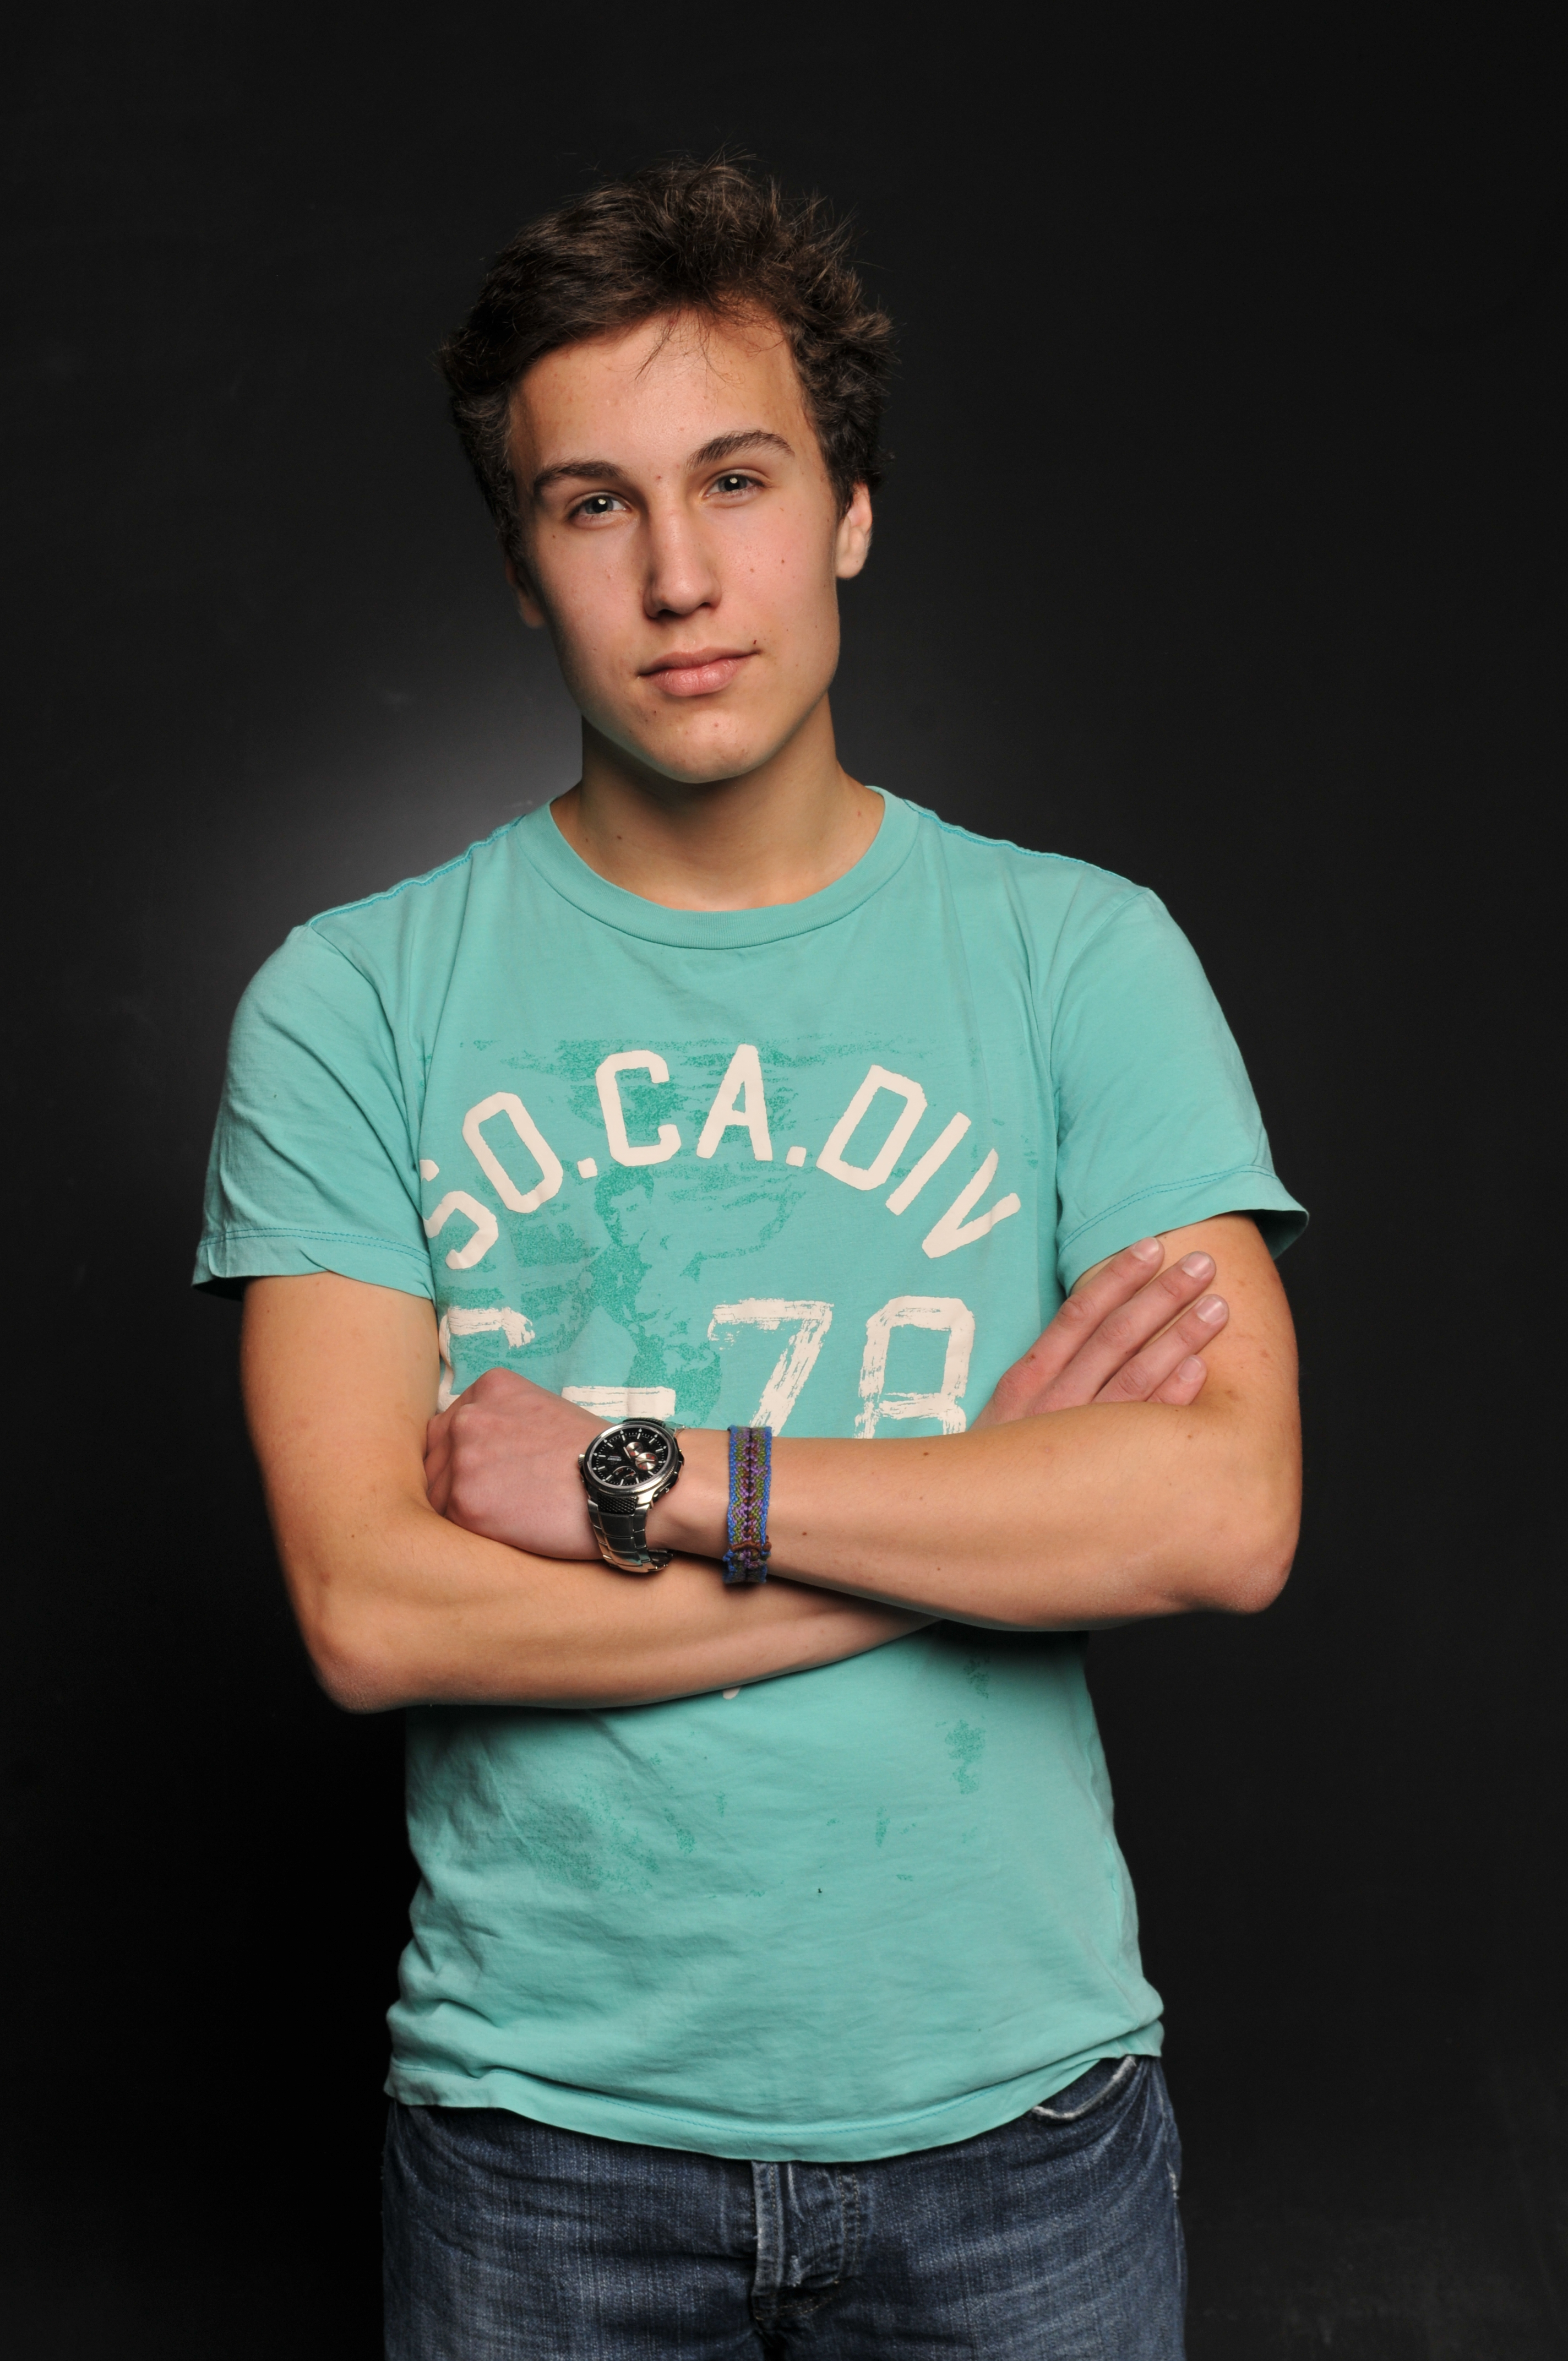
\includegraphics[scale=0.2]{3Engineering/5Team_meetings/days_of_meetings/2015.12.05/images/03}}
		\caption{Beam for operating the climbers (closed)}
		\label{Alpinists1.1}
	\end{minipage}
	\hfill
	\begin{minipage}[h]{0.47\linewidth}
		\center{\includegraphics[scale=0.2]{3Engineering/5Team_meetings/days_of_meetings/2015.12.05/images/04}}
		\caption{Beam for operating the climbers (opened)}
		\label{Alpinists1.2}
	\end{minipage}
\end{figure}